% =====================================================================================================
% A1 PORTRAIT poster (59.4 x 84.1 cm). Four asymmetric quadrants under a title band and an abstract:
%   top-left    1  Background: Muninn                  | top-right    3  Proposed approach
%   bottom-left 2  Muninn on flow matching -> the error | bottom-right 4  Results on a Maze2D planner
% Build: latexmk -pdf poster.tex   (Overleaf: pdfLaTeX).   Figures: python scripts/poster_figures.py
% Body text ~19 pt (= ~26 pt on A0). Grey dashed boxes are figures still to produce (the box says how).
% =====================================================================================================
\documentclass[final]{beamer}
\usepackage[size=custom,width=59.4,height=84.1,scale=0.75]{beamerposter}
\usefonttheme{professionalfonts}
\usefonttheme{serif}
\usepackage[T1]{fontenc}
\usepackage{newtxtext,newtxmath}   % Times-like text + matching math; sans = TeX Gyre Heros (headings)
\usepackage{amsmath,bm}
\usepackage{graphicx,booktabs,multicol,tikz}
\usepackage[most]{tcolorbox}
\usepackage{algpseudocode}
\usetikzlibrary{arrows.meta,decorations.pathreplacing,calc}

% ------------------------------------------------------------------------------------- colours / style
\definecolor{navy}{HTML}{1F3A5F}
\definecolor{ink}{HTML}{111111}
\definecolor{ink2}{HTML}{4A4A46}
\definecolor{rulegray}{HTML}{C9C8C3}
\definecolor{boxgray}{HTML}{F2F3F5}
\definecolor{blue}{HTML}{2A78D6}    % FewSteps AB2
\definecolor{orange}{HTML}{EB6834}  % ours
\definecolor{aqua}{HTML}{1BAF7A}    % Muninn
\setbeamercolor{normal text}{fg=ink}
\setbeamercolor{background canvas}{bg=white}
\setbeamertemplate{navigation symbols}{}
\setbeamertemplate{itemize items}{\color{navy}\raisebox{0.18ex}{\scalebox{0.7}{$\blacksquare$}}}
\setbeamertemplate{enumerate items}{\color{navy}\sffamily\bfseries\insertenumlabel.}
\setbeamersize{text margin left=0cm, text margin right=0cm}
\setlength{\parskip}{0.18cm}
\setlength{\abovedisplayskip}{0.2cm}\setlength{\belowdisplayskip}{0.2cm}
\setlength{\abovedisplayshortskip}{0.1cm}\setlength{\belowdisplayshortskip}{0.2cm}

% section / subsection headings
\newcommand{\psection}[2]{\par
  \begin{tcolorbox}[enhanced, colback=navy, colframe=navy, sharp corners, boxrule=0pt, nobeforeafter,
    left=0.4cm, right=0.4cm, top=0.07cm, bottom=0.07cm]
  {\sffamily\bfseries\LARGE\color{white}#1\hskip0.6em#2}
  \end{tcolorbox}\par\vskip0.05cm}
\newcommand{\sub}[1]{\par\vskip0.08cm{\sffamily\bfseries\large\color{navy}#1}\par\vskip0.02cm}
% numbered figure / table captions
\newcounter{fig}\newcounter{tab}
\newcommand{\figcap}[1]{\refstepcounter{fig}\par\vskip0.06cm{\small{\sffamily\bfseries Figure~\thefig.}\ #1}\par}
\newcommand{\tabcap}[1]{\refstepcounter{tab}\par{\small{\sffamily\bfseries Table~\thetab.}\ #1}\par\vskip0.06cm}
% statement boxes (propositions) and algorithms
\newtcolorbox{statement}[1]{enhanced, colback=boxgray, colframe=navy, boxrule=0pt, leftrule=4pt, arc=0pt,
  left=0.4cm, right=0.4cm, top=0.18cm, bottom=0.18cm, before upper={{\sffamily\bfseries\color{navy}#1}\ }}
\newtcolorbox{algbox}[1]{enhanced, colback=white, colframe=ink2, boxrule=0pt, toprule=1.5pt, bottomrule=1.5pt,
  arc=0pt, left=0.15cm, right=0.15cm, top=0.1cm, bottom=0.06cm, fontupper=\small,
  title={\small\sffamily\bfseries #1}, coltitle=ink, colbacktitle=white, titlerule=0.8pt, titlerule style=ink2,
  toptitle=0.04cm, bottomtitle=0.06cm}
% placeholder for a figure that still has to be produced: #1 width, #2 height, #3 content, #4 how
\newcommand{\placeholder}[4]{\tikz{\node[draw=ink2, dashed, line width=1.5pt, fill=boxgray, minimum width=#1,
  minimum height=#2, text width=\dimexpr#1-1.0cm\relax, align=left, inner sep=0.45cm]
  {{\sffamily\bfseries\color{orange} Figure to produce.}\ #3\\[0.15cm]{\footnotesize\color{ink2}\textbf{How:} #4}};}}
\algrenewcommand\algorithmiccomment[1]{\hfill{\color{ink2}$\triangleright$~#1}}
\algrenewcommand\alglinenumber[1]{{\footnotesize\color{ink2}#1}}

% ------------------------------------------------------------------------------------------- geometry
\newlength{\margin}\setlength{\margin}{1.6cm}
\newlength{\colgap}\setlength{\colgap}{1.3cm}
\newlength{\leftw}\setlength{\leftw}{27.0cm}
\newlength{\rightw}\setlength{\rightw}{\dimexpr\paperwidth-2\margin-\colgap-\leftw\relax}
\newlength{\bodyh}\setlength{\bodyh}{66.8cm}
\newcommand{\quadrule}{\par\vskip0.25cm}

\begin{document}
\begin{frame}[t]

% =============================================================================================== HEADER
\begin{tcolorbox}[enhanced, colback=navy, colframe=navy, sharp corners, boxrule=0pt, width=\paperwidth,
  left=\margin, right=\margin, top=0.75cm, bottom=0.65cm, nobeforeafter]
\begin{minipage}[c]{6.0cm}\centering
  \tikz\node[draw=white, line width=1pt, dashed, minimum width=5.6cm, minimum height=3.4cm, text=white,
    font=\small\sffamily, align=center] {institution\\ logo};
\end{minipage}\hfill
\begin{minipage}[c]{\dimexpr\paperwidth-2\margin-13cm\relax}\centering\color{white}\sffamily
  {\fontsize{52}{60}\selectfont\bfseries Revisiting Certified Step Caching\\[0.05cm] for Flow-Matching Planners}\\[0.45cm]
  {\LARGE Aymane Hamdaoui$^{1}$\qquad Théo Palagi$^{1}$}\\[0.25cm]
  {\large\color{white!80!navy}$^{1}$MVA - ENS \qquad
   \texttt{\{first.last\}@telecom-paris.fr}}
\end{minipage}\hfill
\begin{minipage}[c]{6.0cm}\centering
  \tikz\node[draw=white, line width=1pt, dashed, minimum width=5.6cm, minimum height=3.4cm, text=white,
    font=\small\sffamily, align=center] {lab / partner\\ logo};
\end{minipage}
\end{tcolorbox}

% ============================================================================================= ABSTRACT
\vskip0.45cm
\hskip\margin\begin{minipage}{\dimexpr\paperwidth-2\margin\relax}
\begin{tcolorbox}[enhanced, colback=boxgray, colframe=boxgray, arc=0pt, boxrule=0pt, left=0.6cm, right=0.6cm,
  top=0.3cm, bottom=0.3cm]
{\sffamily\bfseries\color{navy}Abstract.}\ Diffusion and flow-matching (FM) planners integrate a learned velocity
field at one network evaluation (NFE) per step. Muninn~[1] skips evaluations by reusing cached outputs under a
per-step error budget and certifies the deviation of the final plan. Porting it to FM, we show that (i) its
certificate omits how the rest of the chain amplifies reuse errors, and fails for 22--78\% of samples on toy
problems; (ii) certifying the \emph{final} plan with Learn-then-Test calibration restores validity for any
sampler; (iii) under this common guarantee, a uniform second-order integrator (AB2) needs 5--9$\times$ fewer
NFE than Muninn on a Maze2D planner; (iv) the best adaptive scheme we found, an amplification-aware learned
extrapolation policy, gains only 1.2--1.3$\times$ over certified AB2, and only at tight tolerances.
\end{tcolorbox}
\end{minipage}
\vskip0.5cm

% ================================================================================================= BODY
\hskip\margin
% ------------------------------------------------------------------------------------------ LEFT COLUMN
\begin{minipage}[t][\bodyh][t]{\leftw}\vspace{0pt}

% ----------------------------------------------------------------------------------- 1  Muninn (TL)
\psection{1}{Background: certified caching with Muninn}
A planner draws a plan $\tau\in\mathbb{R}^{H\times n}$ for a context $c=(s_0,g)$ by integrating a learned field
over $N$ steps, $x_{k+1}=\Phi_k(x_k,u_k)$, $u_k=v_\theta(x_k,t_k,c)$: one NFE per step. \textbf{Muninn}~[1]
(Alg.~1, Fig.~\ref{fig:chain}) reuses the cached output when a cheap \emph{probe} (first network block) barely changes: a
split-conformal fit $U(s)$ bounds the reuse error $\lVert e_k\rVert$ from the probe score $s_k$, and reuse goes
on while the bounded cost fits a budget $\eta$. With Lipschitz constants $K_j,L'_k$ of the update (Euler: $K=1$,
$L'=h$) it claims
\begin{equation}
  d(\tau^{\mathrm{full}},\tilde\tau)\le\sum_{k\in\mathcal R}\Gamma L_k\lVert e_k\rVert\le\eta
  \ \ \text{w.p.}\ge1-\alpha,\quad L_k=L'_k\prod_{j>k}K_j ,
\end{equation}
with $\mathcal R$ the reuse steps, $e_k$ the error of the reused output \emph{at the cached state} and
$\Gamma=1/\sqrt H$. Reported: up to $7.7\times$ fewer evaluations, e.g.\ $100\to15.3$ NFE on Maze2D with
Diffuser~[1].

\begin{minipage}[t]{0.497\linewidth}\vspace{0pt}
\begin{algbox}{Algorithm 1\ \ Muninn, one plan [1]}
\begin{algorithmic}[1]
\Require budget $\eta$, bound $U$, weights $L_k$, cacheable $\mathcal T$
\State $B\gets\eta$;\ \ $x\gets x_0\sim\mathcal N(0,I)$
\For{$k=0,\dots,N-1$}
  \State $F_k\gets\Psi(x,t_k,c)$;\ \ $s_k\gets\frac{\lVert F_k-F_{k-1}\rVert_1}{\lVert F_{k-1}\rVert_1+\omega}$ \Comment{probe}
  \State $\hat c_k\gets\Gamma L_k\,U(s_k)$
  \State \textbf{if} $k\in\mathcal T\wedge\hat c_k\le B$: $u\gets u_{\mathrm{cache}}$, $B\gets B-\hat c_k$ \Comment{0~NFE}
  \State \textbf{else}: $u\gets v_\theta(x,t_k,c)$, $u_{\mathrm{cache}}\gets u$ \Comment{1~NFE}
  \State $x\gets\Phi_k(x,u)$
\EndFor
\end{algorithmic}
\end{algbox}
\end{minipage}\hfill
\begin{minipage}[t]{0.49\linewidth}\vspace{0pt}
\centering
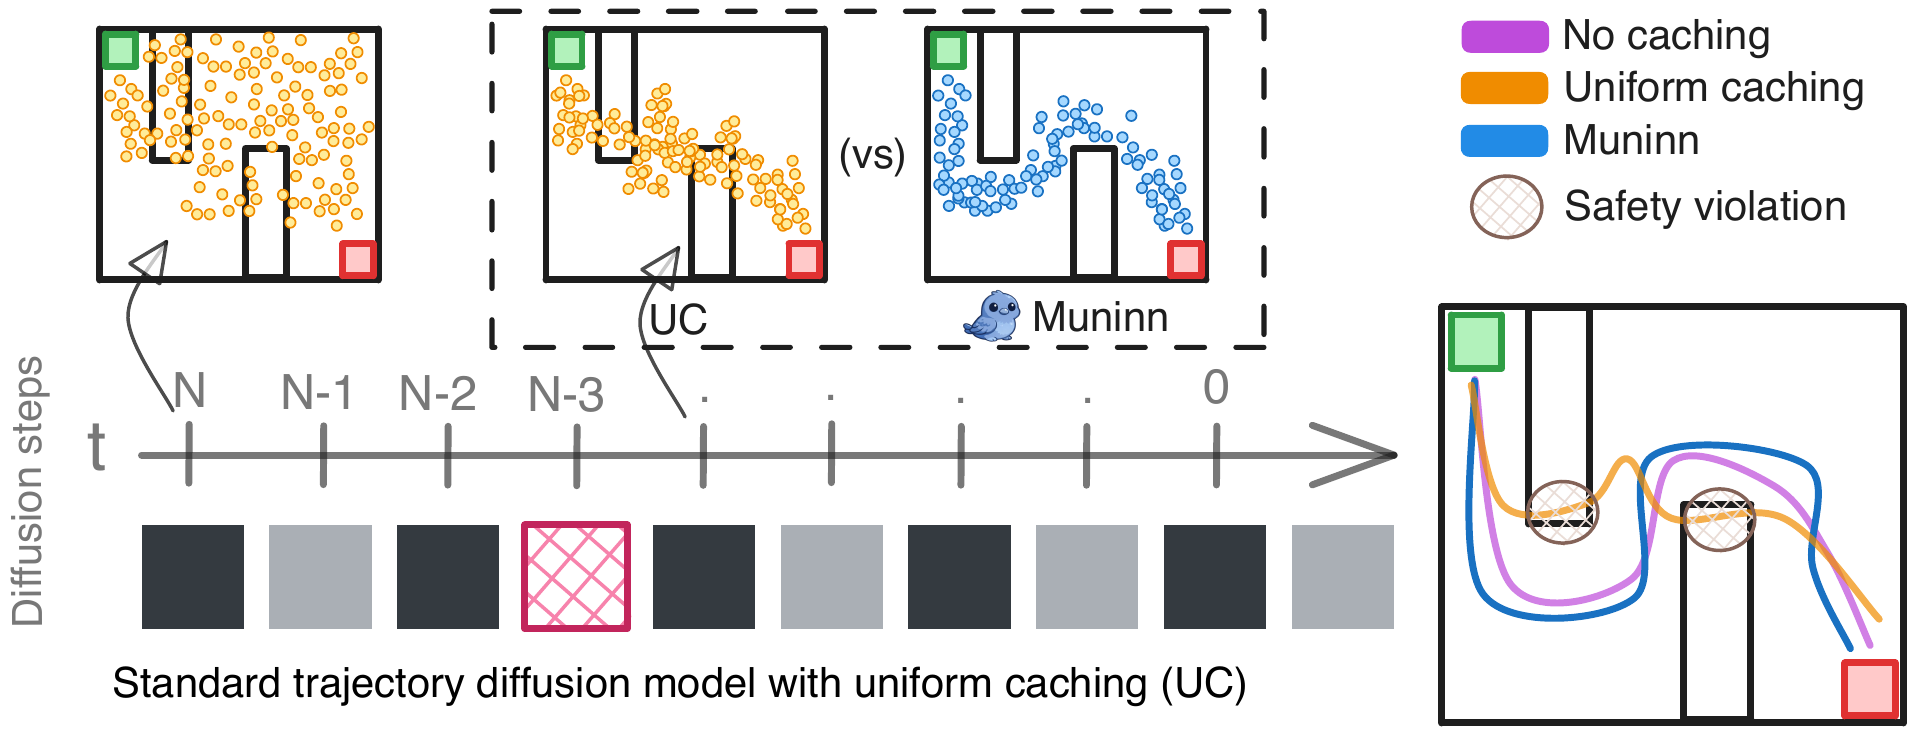
\includegraphics[width=\linewidth]{figures/muninn_fig2_crop.png}
\figcap{Uniform caching (UC) can reuse at a harmful step; Muninn reuses only when safe [1].}\label{fig:chain}
\end{minipage}

\quadrule
% ----------------------------------------------------------------------------- 2  FM experiments (BL)
\psection{2}{Muninn on flow matching: the certificate breaks}
\textbf{Setting.} Conditional optimal-transport FM~[2], $x_t=(1-t)x_0+tx_1$, Euler, $N=100$, on 2D toys
(checkerboard, 8 Gaussians; MLP) where Jacobians and exact solutions are computable. Baseline \emph{FewSteps}:
a uniform grid of $N'<N$ steps, Euler or 2nd-order Adams--Bashforth (AB2, also 1 NFE per step).

\begin{minipage}[t]{0.54\linewidth}\vspace{0pt}
\textbf{(O1) Reuse is inefficient.} At equal mean NFE, FewSteps is 5--15$\times$ closer to the full chain than
Muninn, even on Muninn's own target (Fig.~\ref{fig:pareto}). Knowing the \emph{exact} reuse error does not
help: reusing $v$ for $l$ steps is one Euler step of size $lh$, i.e.\ a non-uniform grid, worse than a
uniform one.\\[0.15cm]
\textbf{(O2) The certificate fails.} With exact errors, Eq.~(1) is violated for 22--78\% of samples
(Table~\ref{tab:valid}); real Muninn exceeds its risk level on checkerboard
($\hat p_{\mathrm{viol}}=0.059$ and $0.083>\alpha=0.05$, 50\,000 test samples).
\end{minipage}\hfill
\begin{minipage}[t]{0.43\linewidth}\vspace{0pt}\centering
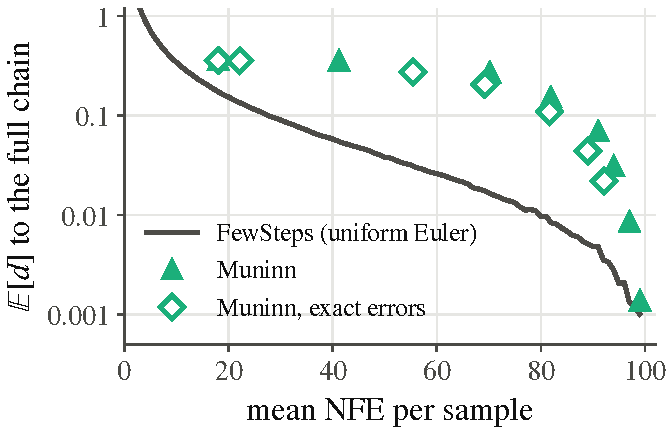
\includegraphics[width=\linewidth]{figures/fig_pareto.pdf}
\figcap{Checkerboard: error vs cost (each Muninn point is one budget $\eta$).}\label{fig:pareto}
\end{minipage}

\vskip0.15cm
\begin{statement}{Proposition 1 (exact error recursion).}
Let $\Delta_k=x^{\mathrm{full}}_k-\tilde x_k$ and $e_k=v_\theta(\tilde x_k)-\tilde u_k$. For Euler,
\begin{equation}
  \Delta_{k+1}=(I+h\bar J_k)\,\Delta_k+h\,e_k\;\;\Longrightarrow\;\;\Delta_N=\sum_k h\,M_{k+1\to N}\,e_k ,
\end{equation}
with $\bar J_k=\int_0^1\partial_x v_\theta(\tilde x_k+s\Delta_k)\,ds$ and
$M_{k+1\to N}=\prod_{j>k}(I+h\bar J_j)\approx G_{k+1\to N}$, the flow Jacobian of the remaining chain.
Eq.~(1) evaluates the network at the cached state, which drops the drift term $h\bar J_k\Delta_k$ ($M=I$).
The valid weight is $L_k=h\lVert M_{k+1\to N}\rVert$.
\end{statement}
\vskip0.12cm
\begin{minipage}[t]{0.49\linewidth}\vspace{0pt}\centering
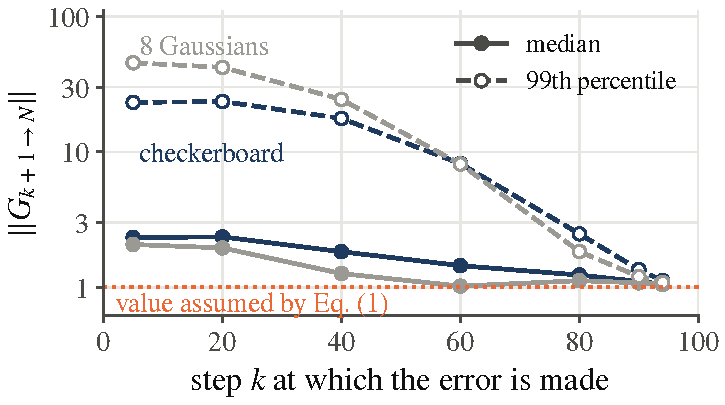
\includegraphics[width=\linewidth]{figures/fig_gnorm.pdf}\\[-0.05cm]{\small(a)}
\end{minipage}\hfill
\begin{minipage}[t]{0.49\linewidth}\vspace{0pt}\centering
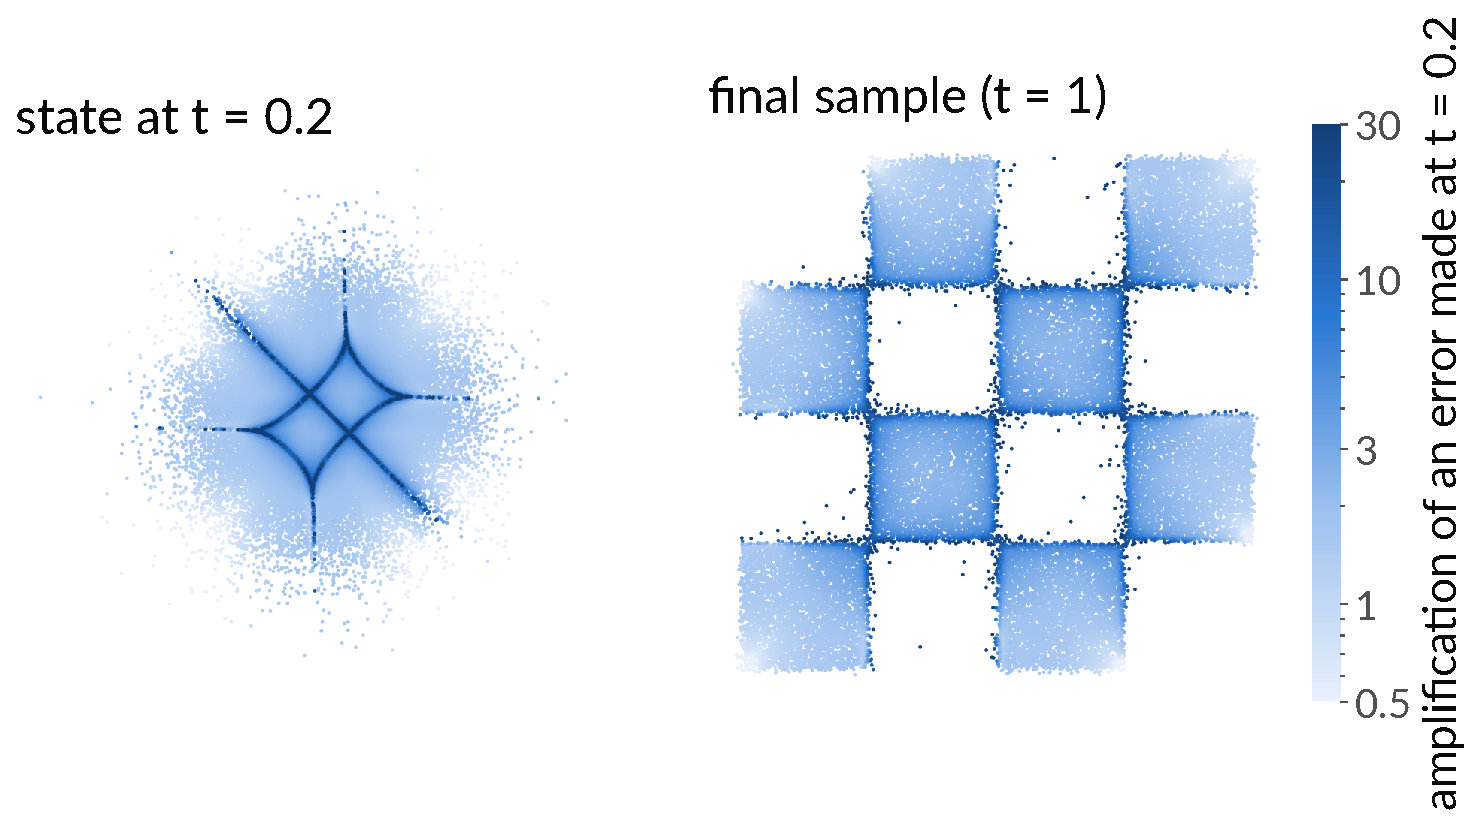
\includegraphics[width=\linewidth]{figures/fig_amplification.pdf}\\[-0.05cm]{\small(b)}
\end{minipage}
\figcap{(a) Amplification $\lVert G_{k+1\to N}\rVert$ of an error made at step $k$: median $\approx2$,
99th percentile 20--45 early in the chain (maximum $\approx10^3$), where Eq.~(1) assumes 1.
(b) Checkerboard, error made at $t=0.2$: amplified 10--30$\times$ near the boundaries between cells.}\label{fig:amp}

\vskip0.12cm
\begin{minipage}[t]{0.5\linewidth}\vspace{0pt}
\begin{statement}{Proposition 2 (Tweedie Jacobian~[6]).}
For CondOT FM, $v(x,t)=\big(\mathbb{E}[x_1\mid x_t=x]-x\big)/(1-t)$, hence
\begin{equation}
  \frac{\partial v}{\partial x}=\frac{1}{1-t}\Big[\frac{t\,\mathrm{Cov}(x_1\mid x_t=x)}{(1-t)^2}-I\Big].
\end{equation}
Errors grow where the endpoint is still uncertain: on the boundaries between modes (Fig.~\ref{fig:amp}b).
\end{statement}
\end{minipage}\hfill
\begin{minipage}[t]{0.47\linewidth}\vspace{0pt}\centering
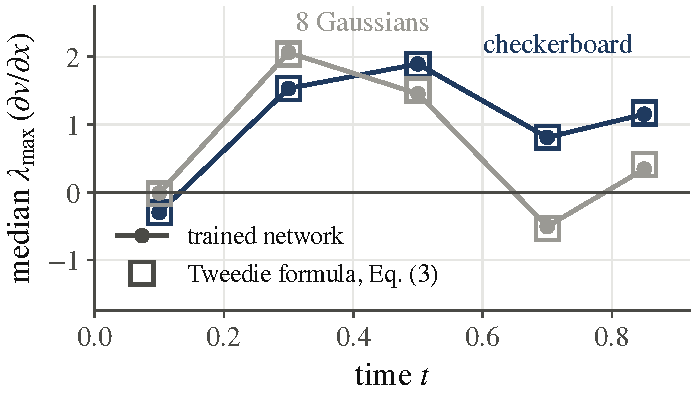
\includegraphics[width=\linewidth]{figures/fig_tweedie.pdf}
\figcap{The trained networks follow Eq.~(3) (correlation 0.98--1.00, $t\in[0.3,0.7]$).}\label{fig:tweedie}
\end{minipage}

\vskip0.15cm
\tabcap{Samples for which the certificate holds (oracle with exact errors, $\eta\in[0.05,1]$). DDPM weights
$K_t=1/\sqrt{\alpha_t}>1$ over-count typical propagation 5--25$\times$, which hides most failures.}\label{tab:valid}
\centering
\begin{tabular}{l c c}
\toprule
model + sampler & Eq.~(1) (paper's weights) & with drift terms (Prop.~1)\\
\midrule
FM + Euler, checkerboard & 21.6--23.4\% & 99.9--100\%\\
FM + Euler, 8 Gaussians  & 77.6--90.2\% & 100\%\\
VP + DDPM, checkerboard  & 95.6--98.7\% & 100\%\\
VP + DDIM, checkerboard  & 93.1--98.1\% & 100\%\\
\bottomrule
\end{tabular}

\end{minipage}%
\hskip\colgap
% ----------------------------------------------------------------------------------------- RIGHT COLUMN
\begin{minipage}[t][\bodyh][t]{\rightw}\vspace{0pt}

% --------------------------------------------------------------------------------- 3  Proposition (TR)
\psection{3}{Proposed approach}
\sub{3.1\ \ Certify the final plan, end to end}
Treat a sampler with one knob $\lambda\in\Lambda$ (step count $N'$, threshold $\tau$, Muninn's budget) as a
black box. On $n$ calibration pairs $(x_0,c)$ count $k_\lambda=\#\{i:d_i(\lambda)>\eta\}$, with $d$ measured to
the exact solution $x^\star$ (RK4-400), and certify $\lambda$ by a Learn-then-Test~[4] binomial test:
\begin{equation}
  p_\lambda=\mathbb{P}\big[\mathrm{Bin}(n,\alpha)\le k_\lambda\big]\le\delta/\lvert\Lambda\rvert .
\end{equation}
Then, w.p.\ $\ge1-\delta$ over calibration, the cheapest certified $\hat\lambda$ satisfies
\begin{equation}
  \mathbb{P}_{x_0,c}\big[d(\hat x_{\hat\lambda},x^\star)>\eta\big]\le\alpha .
\end{equation}
No Lipschitz constant, no union bound over steps: valid for any sampler, Muninn included, and every method
buys the same guarantee.

\sub{3.2\ \ Spend NFE where errors are amplified}
Three changes suggested by \S2: (i) a second-order base grid, AB2:
$x_{k+1}=x_k+h(\tfrac32u_k-\tfrac12u_{k-1})$; (ii) \emph{extrapolate} instead of reusing,
$\hat u_k=u_b+\frac{t_k-t_b}{t_b-t_a}(u_b-u_a)$ from the last two computed velocities (Fig.~\ref{fig:extrap});
(iii) decide with the \emph{amplified} cost of Prop.~1 (Alg.~2):
\begin{equation}
  c_k=h\,\lVert G_{k+1\to N}\,e_k\rVert,\qquad\text{extrapolate}\iff\hat c_k\le\tau\ \text{and lag}<10 .
\end{equation}
\textbf{A threshold, not a budget.} If $\Delta_N\approx\sum_k h\,G\,e_k$, minimising the calls subject to
$\sum_kc_k\le B$ has the Lagrangian $\sum_k\mathbf{1}[\mathrm{compute}_k]+\mu\,c_k\mathbf{1}[\mathrm{extrap}_k]$,
minimised step by step by $c_k\le1/\mu=\tau$. Muninn's first-come budget needed 3--8$\times$ more NFE (oracle study).

\begin{minipage}[t]{0.44\linewidth}\vspace{0.1cm}\centering
\resizebox{\linewidth}{!}{%
\begin{tikzpicture}[x=1cm, y=1.25cm, every node/.style={font=\sffamily\large}]
  \draw[-{Stealth}, line width=1.2pt, ink2] (0,0) -- (10.4,0) node[below left] {$t$};
  \draw[-{Stealth}, line width=1.2pt, ink2] (0,0) -- (0,4.3);
  \node[rotate=90, anchor=south, text=ink2] at (-0.15,2.15) {velocity};
  \draw[line width=2.4pt, ink, domain=0.5:9.4, samples=60] plot (\x, {0.6+0.42*\x-0.01*\x*\x});
  \draw[dashed, line width=2pt, aqua] (5.5,2.6075) -- (8,2.6075);
  \draw[dashed, line width=2pt, orange] (4,2.12) -- (8,3.42);
  \draw[dotted, line width=1.2pt, ink2] (8,0) -- (8,2.45);
  \node[below, text=ink2] at (8,0) {$t_k$};
  \fill[navy] (4,2.12) circle (0.16) node[below right=1pt, text=navy] {$u_a$};
  \fill[navy] (5.5,2.6075) circle (0.16) node[below right=1pt, text=navy] {$u_b$};
  \fill[ink] (8,3.32) circle (0.14);
  \draw[aqua, line width=2.4pt, fill=white] (8,2.6075) circle (0.16);
  \draw[orange, line width=2.4pt, fill=white] (8,3.42) circle (0.16);
  \draw[decorate, decoration={brace, amplitude=6pt, mirror}, line width=1.6pt, aqua] (8.35,2.62) -- (8.35,3.28)
     node[midway, right=8pt, yshift=-0.2cm, text=aqua, align=left] {reuse\\error};
  \draw[line width=1.2pt, orange] (7.8,3.45) -- (7.0,3.95) node[left, text=orange] {extrapolation error};
  \node[anchor=south west, text=ink2, font=\sffamily\normalsize] at (0.3,0.12) {$\bullet$ computed\quad $\circ$ predicted};
\end{tikzpicture}}
\figcap{Reuse (Muninn) vs linear extrapolation (ours) of the velocity at step $k$.}\label{fig:extrap}
\end{minipage}\hfill
\begin{minipage}[t]{0.53\linewidth}\vspace{0pt}
\begin{algbox}{Algorithm 2\ \ Ours, one plan}
\begin{algorithmic}[1]
\Require threshold $\tau$, cost regressor $f$, max lag $m$
\State compute $u_0,u_1$ (first step: Euler)
\For{$k=2,\dots,N-1$}
  \State $\hat u_k\gets u_b+\frac{t_k-t_b}{t_b-t_a}(u_b-u_a)$
  \State $\hat c_k\gets\exp f(\text{free signals}_k)$
  \State \textbf{if} $\hat c_k\le\tau$ \textbf{and} lag $<m$: $u_k\gets\hat u_k$ \Comment{0~NFE}
  \State \textbf{else}: $u_k\gets v_\theta(x_k,t_k,c)$ \Comment{1~NFE}
  \State $x_{k+1}\gets x_k+h(\tfrac32u_k-\tfrac12u_{k-1})$
\EndFor
\end{algorithmic}
\end{algbox}
\end{minipage}

\sub{3.3\ \ Learning the cost}
$c_k$ depends on the unknown error and on the future, so an MLP regresses $\log c_k$ offline from \emph{free}
signals ($t$, lag, $\lVert u\rVert$, rates of change of $u$ and of the endpoint $x+(1-t)u$), optionally plus
Muninn's probe: 196\,000 rows from 2000 ghost chains, targets $G_{k+1\to N}e_k$ by finite-difference
Jacobian--vector products (within 0.2\% of autodiff).

\vfill\quadrule
% ------------------------------------------------------------------------------------- 4  Results (BR)
\psection{4}{Results on a Maze2D planner}
\begin{minipage}[t]{0.47\linewidth}\vspace{0pt}
\textbf{Setup.} D4RL Maze2D U-maze~[5], stitched episodes cut into $H=128$-step windows of
$(x,y,\dot x,\dot y,a_x,a_y)$. Temporal U-Net (3.2\,M parameters, Diffuser-style~[3]), CondOT FM, conditioned
on $c=(s_0,g)$ by FiLM, EMA 0.999. Euler-100 plans: start / goal error 0.017 / 0.020, 0.9\% with a jump,
0.05\% touching a wall. Certification: 4000 calibration and 20\,000 test pairs $(x_0,c)$,
$\alpha=\delta=0.05$, reference RK4-400; our policy: 3 seeds.
\end{minipage}\hfill
\begin{minipage}[t]{0.215\linewidth}\vspace{0pt}\centering
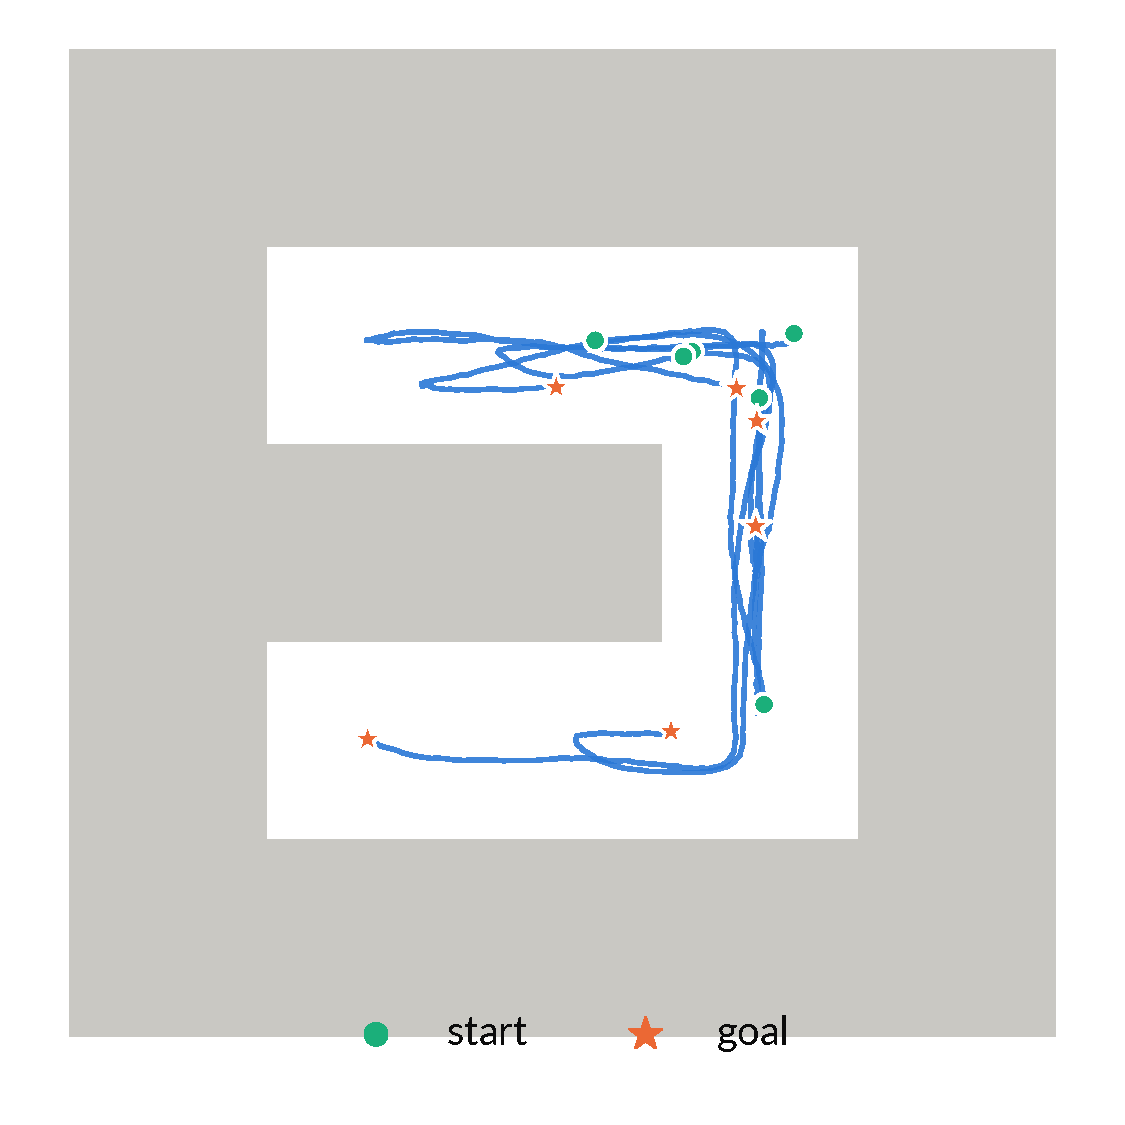
\includegraphics[width=\linewidth]{figures/fig_maze.pdf}
\figcap{Plans for random $(s_0,g)$.}\label{fig:maze}
\end{minipage}\hfill
\begin{minipage}[t]{0.285\linewidth}\vspace{0pt}
\placeholder{\linewidth}{7.3cm}{Same contexts, plans of the exact solver, certified Muninn, AB2 and ours,
with NFE and $d$.}{new script sampling each certified setting (\texttt{certified\_compare/}, \texttt{e19/})
on 3--4 contexts; save or retrain the E19 regressor first.}
\end{minipage}

\vskip0.1cm
\begin{minipage}[t]{0.49\linewidth}\vspace{0pt}\centering
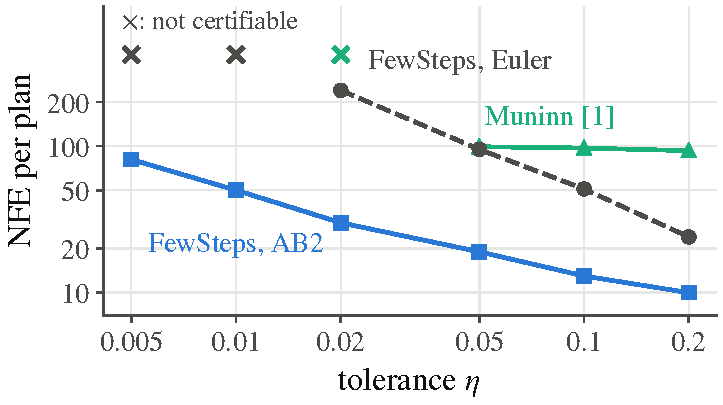
\includegraphics[width=\linewidth]{figures/fig_e18.pdf}\\[-0.05cm]{\small(a) Muninn vs FewSteps}
\end{minipage}\hfill
\begin{minipage}[t]{0.49\linewidth}\vspace{0pt}\centering
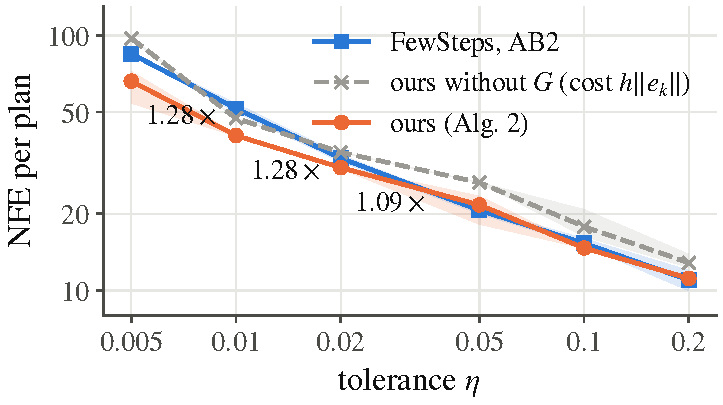
\includegraphics[width=\linewidth]{figures/fig_e19.pdf}\\[-0.05cm]{\small(b) ours vs FewSteps AB2}
\end{minipage}
\figcap{NFE needed for the same certified guarantee $\mathbb{P}[d>\eta]\le0.05$. (a) $\times$: no setting
certifies. (b) Mean of 3 seeds, band = min--max; labels: speed-up over AB2.}

\vskip0.15cm
\begin{minipage}[t]{0.55\linewidth}\vspace{0pt}
\tabcap{Certified NFE per plan, U-maze.}
\centering\small
\begin{tabular}{r rrrr r}
\toprule
$\eta$ & Euler & Muninn & AB2 & \textbf{ours} & gain\\
\midrule
0.005 & -- & -- & 84.7 & \textbf{66.1} & \textbf{1.28}$\times$\\
0.01  & -- & -- & 51.7 & \textbf{40.5} & \textbf{1.28}$\times$\\
0.02  & 240 & -- & 33.0 & \textbf{30.3} & 1.09$\times$\\
0.05  & 95 & 99 & \textbf{20.7} & 21.7 & 0.95$\times$\\
0.1   & 51 & 97 & 15.3 & \textbf{14.7} & 1.04$\times$\\
0.2   & 24 & 93 & \textbf{11.0} & 11.2 & 0.98$\times$\\
\bottomrule
\end{tabular}\\[0.08cm]
{\footnotesize\raggedright --: not certifiable. AB2, ours: mean of 3 seeds. All test violation rates
$\le5.1\%$.\par}
\end{minipage}\hfill
\begin{minipage}[t]{0.42\linewidth}\vspace{0pt}
\tabcap{Summary across settings.}
\centering\small
\begin{tabular}{l ccc}
\toprule
 & chk. & 8G & U-maze\\
\midrule
state dimension & 2 & 2 & 768\\
Eq.~(1) holds & 22\% & 78\% & --\\
Muninn / AB2$^{a}$ & 9.7$\times$ & 9.3$\times$ & 7.5$\times$\\
oracle gain$^{b}$ & 1.45$\times$ & 1.47$\times$ & --\\
ours, gain$^{b}$ & 1.28$\times$ & 1.24$\times$ & 1.28$\times$\\
probe helps & no & no & no\\
\bottomrule
\end{tabular}\\[0.08cm]
{\footnotesize\raggedright $^{a}$NFE ratio at $\eta=0.1$. $^{b}$Over certified AB2, best $\eta$.\par}
\end{minipage}

\vfill\vskip0.25cm
\begin{tcolorbox}[enhanced, colback=white, colframe=navy, boxrule=1.5pt, arc=0pt, left=0.35cm, right=0.35cm,
  top=0.06cm, bottom=0.06cm, title={\sffamily\bfseries Conclusions}, colbacktitle=navy, coltitle=white,
  toptitle=0.04cm, bottomtitle=0.04cm]
\begin{enumerate}
  \item Muninn's certificate omits error amplification (Prop.~1): on FM it fails for up to 78\% of samples,
    and DDPM weights only mask the gap.
  \item Certifying the final plan (Eqs.~4--5) is simple, valid for any sampler, and makes comparisons fair.
  \item Under the same guarantee, uniform AB2 needs 5--9$\times$ fewer NFE than Muninn (toys: 6--14$\times$).
  \item Per-step adaptivity is worth little: the best realistic policy gains 1.2--1.3$\times$, only at tight
    tolerances; Muninn's probe adds nothing.
\end{enumerate}
{\small\textbf{Limitations.} One maze, one backbone; closeness to the exact plan, not closed-loop success.}
\end{tcolorbox}

\end{minipage}

% =============================================================================================== FOOTER
\vfill
\hskip\margin\begin{minipage}{\dimexpr\paperwidth-2\margin\relax}
{\color{rulegray}\hrule height 1.2pt}\vskip0.2cm
\begin{multicols}{4}\footnotesize\setlength{\parskip}{0.04cm}\raggedright
\textbf{References}\par
[1] G.~Puthumanaillam, H.~Jiang, R.~Hernandez, J.~Fuentes, P.~Padrao, L.~Bobadilla, M.~Ornik. Muninn: your
trajectory diffusion model but faster. RSS 2026, arXiv:2605.09999.\par
[2] Y.~Lipman, R.~T.~Q.~Chen, H.~Ben-Hamu, M.~Nickel, M.~Le. Flow matching for generative modeling. ICLR 2023.\par
[3] M.~Janner, Y.~Du, J.~B.~Tenenbaum, S.~Levine. Planning with diffusion for flexible behavior synthesis.
ICML 2022.\par
[4] A.~N.~Angelopoulos, S.~Bates, E.~J.~Cand\`es, M.~I.~Jordan, L.~Lei. Learn then test: calibrating predictive
algorithms to achieve risk control. arXiv:2110.01052, 2021.\par
[5] J.~Fu, A.~Kumar, O.~Nachum, G.~Tucker, S.~Levine. D4RL: datasets for deep data-driven reinforcement
learning. arXiv:2004.07219, 2020.\par
[6] B.~Efron. Tweedie's formula and selection bias. JASA 106(496), 2011.\par
\textbf{Acknowledgements.} [placeholder]\quad \textbf{Code.} ![https://github.com/theoplg/Muninn-X]\par
\end{multicols}
\end{minipage}
\vskip0.6cm
\end{frame}
\end{document}
